\documentclass{ee208report}

\title{Lab Report 12}

\begin{document}

\begin{CJK}{UTF8}{gbsn}
    \maketitle
\end{CJK}

\begin{multicols*}{2}

\section{Introduction}

In this lab report, we present our implementation of
SIFT\cite{lowe2004distinctive} through a combination of OpenCV's built-in
functions and techniques suggested in the paper. SIFT, short for scale invariant
feature transform, describe an image by its distinctive features in the form of
keypoints and associated feature descriptors.

The report centers around the implementation and performance of SIFT. We decompose SIFT into a series of steps in Section~\ref{s:anatomy} and explain our implementation for each step in the sections that follow.

\section{Anatomy of SIFT}
\label{s:anatomy}

SIFT involves the following steps\footnote{\underline{\href{http://aishack.in/
tutorials/sift-scale-invariant-feature-transform-introduction/}{SIFT: Theory and
Practice: Introduction - AI Shack}}}:

\begin{enumerate}
    \item \textbf{Constructing a scale space} This is the initial preparation.
    You create internal representations of the original image to ensure scale
    invariance. This is done by generating a "scale space".
    \item \textbf{LoG Approximation} The Laplacian of Gaussian is great for
    finding interesting points (or key points) in an image. But it's
    computationally expensive. So we cheat and approximate it using the
    representation created earlier.
    \item \textbf{Finding keypoints} With the super fast approximation, we now
    try to find key points. These are maxima and minima in the Difference of
    Gaussian image we calculate in step 2
    \item \textbf{Eliminate bad key points} Edges and low contrast regions are
    bad keypoints. Eliminating these makes the algorithm efficient and robust. A
    technique similar to the Harris Corner Detector is used here.
    \item \textbf{Assigning an orientation to the keypoints} An orientation is
    calculated for each key point. Any further calculations are done relative to
    this orientation. This effectively cancels out the effect of orientation,
    making it rotation invariant.
    \item \textbf{Generate SIFT features} Finally, with scale and rotation
    invariance in place, one more representation is generated. This helps
    uniquely identify features. Lets say you have 50,000 features. With this
    representation, you can easily identify the feature you're looking for
    (say, a particular eye, or a sign board).
\end{enumerate}

Due to lack of time, we didn't find keypoints with pyramids of images but used
the built-in \texttt{goodFeaturesToTrack()} to directly retrieve keypoints
instead.

\section{Implementation}

Following the outline laid out in the previous section, we present our
implementation of SIFT.

\subsection{Finding keypoints}

\texttt{goodFeaturesToTrack()} is configured to return all found keypoints:

\begin{minted}{python}
    keypoints = cv.goodFeaturesToTrack(
        img, 0, 0.01, 10).reshape(-1, 2)
\end{minted}

\subsection{Assigning orientation}

For each keypoint, a $5 \times 5$ window around the keypoint is used to find the
keypoint orientation. Since all keypoints returned by
\texttt{goodFeaturesToTrack()} have integer coordinates, no interpolation is
needed.

The magnitudes and angles of gradients that are not on the border are calculated
first.

\begin{minted}{python}
    dy = (img[2:, 1:-1].astype(np.int32)
        - img[:-2, 1:-1])
    dx = (img[1:-1, 2:].astype(np.int32)
        - img[1:-1, :-2])
    # if the image is m * n, the mags and angles
    # array are (m - 2) * (n - 2)
    mags = np.sqrt(dx * dx + dy * dy)
    angles = np.rad2deg(np.arctan2(dy, dx))
\end{minted}

\begin{figure}[H]
    \centering
    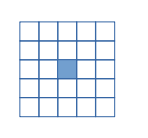
\includegraphics{images/keypoint_window.png}
    \caption{$5 \times 5$ grids for finding orientation. Each cell is a pixel.
        The cell representing the keypoint is shaded.}
    \label{fig:keypoint-window}
\end{figure}

Note that integers must be cast to an appropriate signed type before subtraction
to prevent overflow. Then, angles are converted from
$(-180^\circ, 180^\circ]$ to $[0^\circ, 360^\circ)$.

\begin{minted}{python}
    # convert angle representation from
    # (-180, 180] to [0, 360)
    angles += ((angles < 0).astype(np.int16)
        * 360)
\end{minted}

\bibliographystyle{plain}
\bibliography{lowe2004distinctive}

\end{multicols*}

\end{document}
